\documentclass[../../index.tex]{subfiles}

\begin{document}
\chapter{Introduction}
In particle physics we are concerned about small objects and their interactions.
Since the 1970 the dynamics of these tiny pieces are best described by the Standard Model (SM).

The SM contains two groups of fermionic, Spin 1/2 particles. The former group,
the Leptons consist of: the electron ($e$), the muon ($\mu$), the tau ($\tau$)
and their corresponding neutrinos $\nu_e$, $\nu_\mu$ and $\nu_\tau$. The latter
group, the Quarks contain: $u$, $d$ (up and down, the so called light quarks ),
$s$ (strange), $c$ (charm), $b$ (bottom or beauty) and $t$ (top or truth). The SM
furthermore differenciates between three fundamental forces (and its carriers):
the electromagnetic ($\gamma$ photon), weak ($Z$- or $W$-Boson) and strong ($g$
gluon) interactions. The before mentioned Leptons solely interact through the
electromagnetic and the weak force (also refered to as electroweak interaction),
whereas the quarks additionally interact through the strong force. A short
summary of the taxonomy of the SM can be seen in \cref{fig:SMTaxonomy}
\begin{figure}
  \centering
  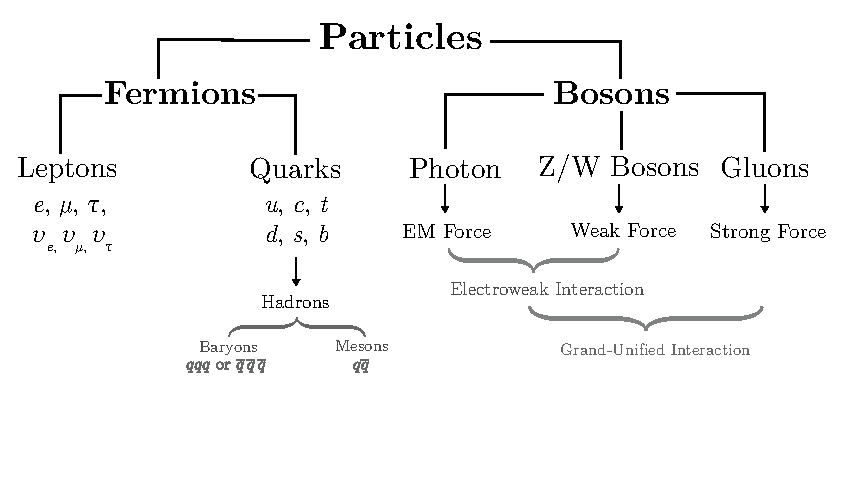
\includegraphics[width=\textwidth]{./images/standardModelTaxonomy.eps}
  \caption{Taxonomy of the Standard Model.}
  \label{fig:SMTaxonomy}
\end{figure}

All of the particles and forces given in the SM are described by a Lagrangian
containing 19 parameters. Ten masses, four CKM-matrix parameters, the QCD vacuum
angle, the Higgs vacuum expectation value and three gauge coupling constants.
Every single parameter has to be fitted from experimental data. Highly accurate
values with low errors are crucial for theoretical calculated predictions. One
of the major error inputs of every theoretical output are uncertainties in these
parameters. In this work we will measure one of these parameters to high
precision: the strong coupling $\alpha_s$, which forms part of the theory of
\textit{quantum chromodynamics} (QCD).

As the name suggest\footnote{Chromo is the greek word for color.} the
force is characterized by the color charge. Every quark has next to its type one
of the three colors blue, red or green. The color force is mediated through
eight gluons, which each being bi-colored\footnote{Each gluon carries a color
  and an anti-color.}, interact with quarks and each other. The strength of the
strong force is given by the coupling constant $\alpha_s$. The strong coupling
varies with energy and contains an exeptional property. It increases with for
low energies\footnote{In contrast to the electromagnetic force, where $\alpha(q^2)$
  decreases!}. This is exclusive for QCD and has two main implications.

The first implication is that, for low energies the coupling is too strong to
isolate quarks. Until now we have not been able to observe an isolated quarks
and all experiments can only measure quark compositions. These bound states are
called \textit{hadrons} and consist of two or three quarks\textit{There exist
  also so-called \textit{Exotic hadrons}, which have more than three valence
  quarks.}, which are refered to as Mesons\footnote{Composite of a quark and an
  anti-quark.} or Baryons \footnote{Composite of three quarks or three
  anti-quarks.} respectively. This
phenomen, of quarks sticking together as hadrons is refered to as \textit{confinement}. 
As the fundamental degrees of freedom of QCD are given by quarks and gluons, but
the observed particles are hadrons we need to introduce the assumption of
\textit{quark-hadron duality}. This means that a physical quantity should be
similarly describable in the hadronic picture or quark-gluon picture and that
both descriptions are equivalent. As we will see in our work quark-hadron
duality is violated for low energies. These so-called \textit{duality
  violations} have an impact on our strong coupling determinations and can be
dealt with either suppression or the inclusion of a model \cite{}. Throughout
this work will favor and argument for the the former approach.

The second implications concerns \textit{perturbation theory} (PT). The lower
the energies we deal with, the higher the value of the strong coupling and the
the contributions of \textit{non-perturbative} (NP) effects. Currently there are
three solutions to deal with NP effects:
\begin{itemize}
  \item \textbf{Chiral Perturbation Theory} (ChPT): Introduced by Weinberg
    \cite{Weinberg1978} in the late seventies ChPT is an effective field theory
    constructed with a Lagrangian symmetric under chiral transformation in the
    limit of massless quarks. It's limitations are based in the chiral symmetry,
    which is only a good approximation for the light quarks u, d and in some
    cases s.
  \item \textbf{Lattice QCD} (LQCD): Is the numerical approach to the strong
    force. Based on the Wilson Loops \cite{Wilson1974} we treat QCD on a finite
    latice instead of continous fields. LQCD has already many applications but
    is limited due to its computational expensice calculations.
  \item \textbf{QCD Sum Rules}: Was also introduced in the late seventies by
    Shifman, Vainstein and Zakharov \cite{Shifman1978,Shifman1978a}. It relates
    the observed hadronic picture to quark-gluon parameters through a dispersion
    relation and the use of the \textit{Operator Product Expansion}, which
    treats NP effect through the definition of vacuum expectation values as the
    so-called \textit{QCD condensates}. It is a precise method for extracting
    the strong coupling $\alpha_s$ at low energies, although limited to
    the uknown higher order contributions of the OPE.
\end{itemize}


In the following (\cref{sec:tauDecays}) we will describe the $\tau$-decays, which
play an essential role in our QCD analysis. Then in \cref{sec:quantumchromodynamics} we want to give more
details of QCD, especially about the coupling constant $\alpha_s(s)$ (which is not
constant at all) and the \textit{QCD sum rules}.


\end{document}